\documentclass[10pt]{acmsiggraph}               % final
%\documentclass[review]{acmsiggraph}      % review
%\documentclass[widereview]{acmsiggraph}  % wide-spaced review
%\documentclass[preprint]{acmsiggraph}    % preprint

%% Uncomment one of the four lines above depending on where your paper is
%% in the conference process. ``review'' and ``widereview'' are for review
%% submission, ``preprint'' is for pre-publication, and ``final'' is for
%% the version to be printed.

%% These two line bring in essential packages: ``mathptmx'' for Type 1 
%% typefaces, and ``graphicx'' for inclusion of EPS figures.

\usepackage{mathptmx}
\usepackage{graphicx}

%% use this for zero \parindent and non-zero \parskip, intelligently.

\usepackage{parskip}

\usepackage{amsmath}

%% If you are submitting a paper to the annual conference, please replace 
%% the value ``0'' below with your OnlineID. If you are not submitting this
%% paper to the annual conference, you may safely leave it at ``0'' -- it 
%% will not be included in the output.

\onlineid{0}

%% need to document this!

\acmformat{print}

%% Paper title.

\title{Segmentation for Fun and Profit\\
\small{July 2006}}

%% Author and Affiliation (single author).

\author{Devin Smith\\Harvey Mudd College\\dsmith@hmc.edu}%\thanks{e-mail: dsmith@hmc.edu}}


%% Keywords that describe your work.

\keywords{clustering, segmentation, sketch}

%%%%%% START OF THE PAPER %%%%%%

\begin{document}

%\teaser{
%	\includegraphics[width=1.5in]{SEGMENTATION.gif}%sample.eps}
%  \caption{Lookit! Lookit!}
%}

%% The ``\maketitle'' command must be the first command after the
%% ``\begin{document}'' command. It prepares and prints the title block.

\maketitle

\section{Abstract}

Lorem ipsum dolor sit amet, consectetur adipisicing elit, sed do eiusmod tempor incididunt ut labore et dolore magna aliqua. Ut enim ad minim veniam, quis nostrud exercitation ullamco laboris nisi ut aliquip ex ea commodo consequat. Duis aute irure dolor in reprehenderit in voluptate velit esse cillum dolore eu fugiat nulla pariatur. Excepteur sint occaecat cupidatat non proident, sunt in culpa qui officia deserunt mollit anim id est laborum.

\section{Problem Statement}

%% The ``\copyrightspace'' command must be the first command after the 
%% start of the first section of the body of your paper. It ensures the
%% copyright space is left at the bottom of the first column on the first
%% page of your paper.

%\copyrightspace

%\begin{itemize}
%\item What is a sketch?
%\item Why are we interested in sketches?
%\item Describe the overall problem we are trying to solve.
%\item Give concise problem that we are trying to solve with segmentation.
%\item Give overview of segmentation component and problem associated with that
%\item Note: Mention that with this segmentation we have more information than most
%do when they are segmenting. We have a label and probability for each stroke to
%supplement segmentation, while other approaches do not.
%\end{itemize}

%Feel I need to talk about the overall project here and what a sketch is.

Frequently during a design process sketches are made because they are quick and simple ways to visually express the design.
Unfortunately, there are not many systems that can recognize the sketch.
Many of the systems that do exist place unnatural restrictions on how the user sketches, such as forcing the user to pause after every symbol has been drawn, imposing a single stroke to symbol correspondance, or imposing that multiple symbols cannot be made with a single stroke.
Our system aims to recognize sketches from the domain of logic circuit diagrams, and ultimately have a sketch recognized and implemented in a circuit simulator without placing any restrictions on users' sketching style.
 %What are some of the problems and difficulties in this domain?

Sketch recognition is more than just recognition.
It usually consists of three main steps: preprocessing, segmentation, and recognition.
Preprocessing takes a sketch and cleans up the data by removing unnecessary points and breaking up the strokes into lines and arcs.
Segmentation partitions the preprocessed sketch.
Recognition takes the parts from segmentation and tries to classify them.

Segmentation, for sketch recognition, is the process of partitioning the strokes of a sketch until a ``correct'' partition is reached.
``Correct'' here is defined in the recognition step when all parts of the partition can be recognized with some amount of certainty.
The simplest way to implement segmentation is to try every partion of the strokes.
While this is very simple, it consumes exponentially time. 
This is why segmentation is arguably the most complex problem in sketch recognition~\cite{pattern}.
For example, given a sketch composed of 20 strokes (a rather small sketch), there are more than 50 trillion items in the search space (the same number of partitions).
Our goal is to use the data and domain specific information to segment a sketch in less than exponential time. 

For the logical circuit diagram domain, a ``correct'' partition would be a partition were there was a part for each component in the diagram.
Consider Figure~\ref{fig:simple}. 
A correct partition of the strokes for this would be \{\{1\} \{2\} \{3 4\} \{5 6 7\} \{8\} \{9\} \{10 11\} \{12 13 14\} \{15 16\} \{17\}\} with the corresponding recognition of AND:\{\{3 4\} \{15 16\}\} OR:\{\{10 11\}\} WIRE:\{\{1\} \{2\} \{5 6 7\} \{8\} \{9\} \{12 13 14\} \{17\}\}. 
This partition may seem relatively trivial to find, yet imagine if the strokes were unordered, overlapping, and inconsistent in size.
Remember, there are no restrictions placed on the user.

\begin{figure}[h]
\centering
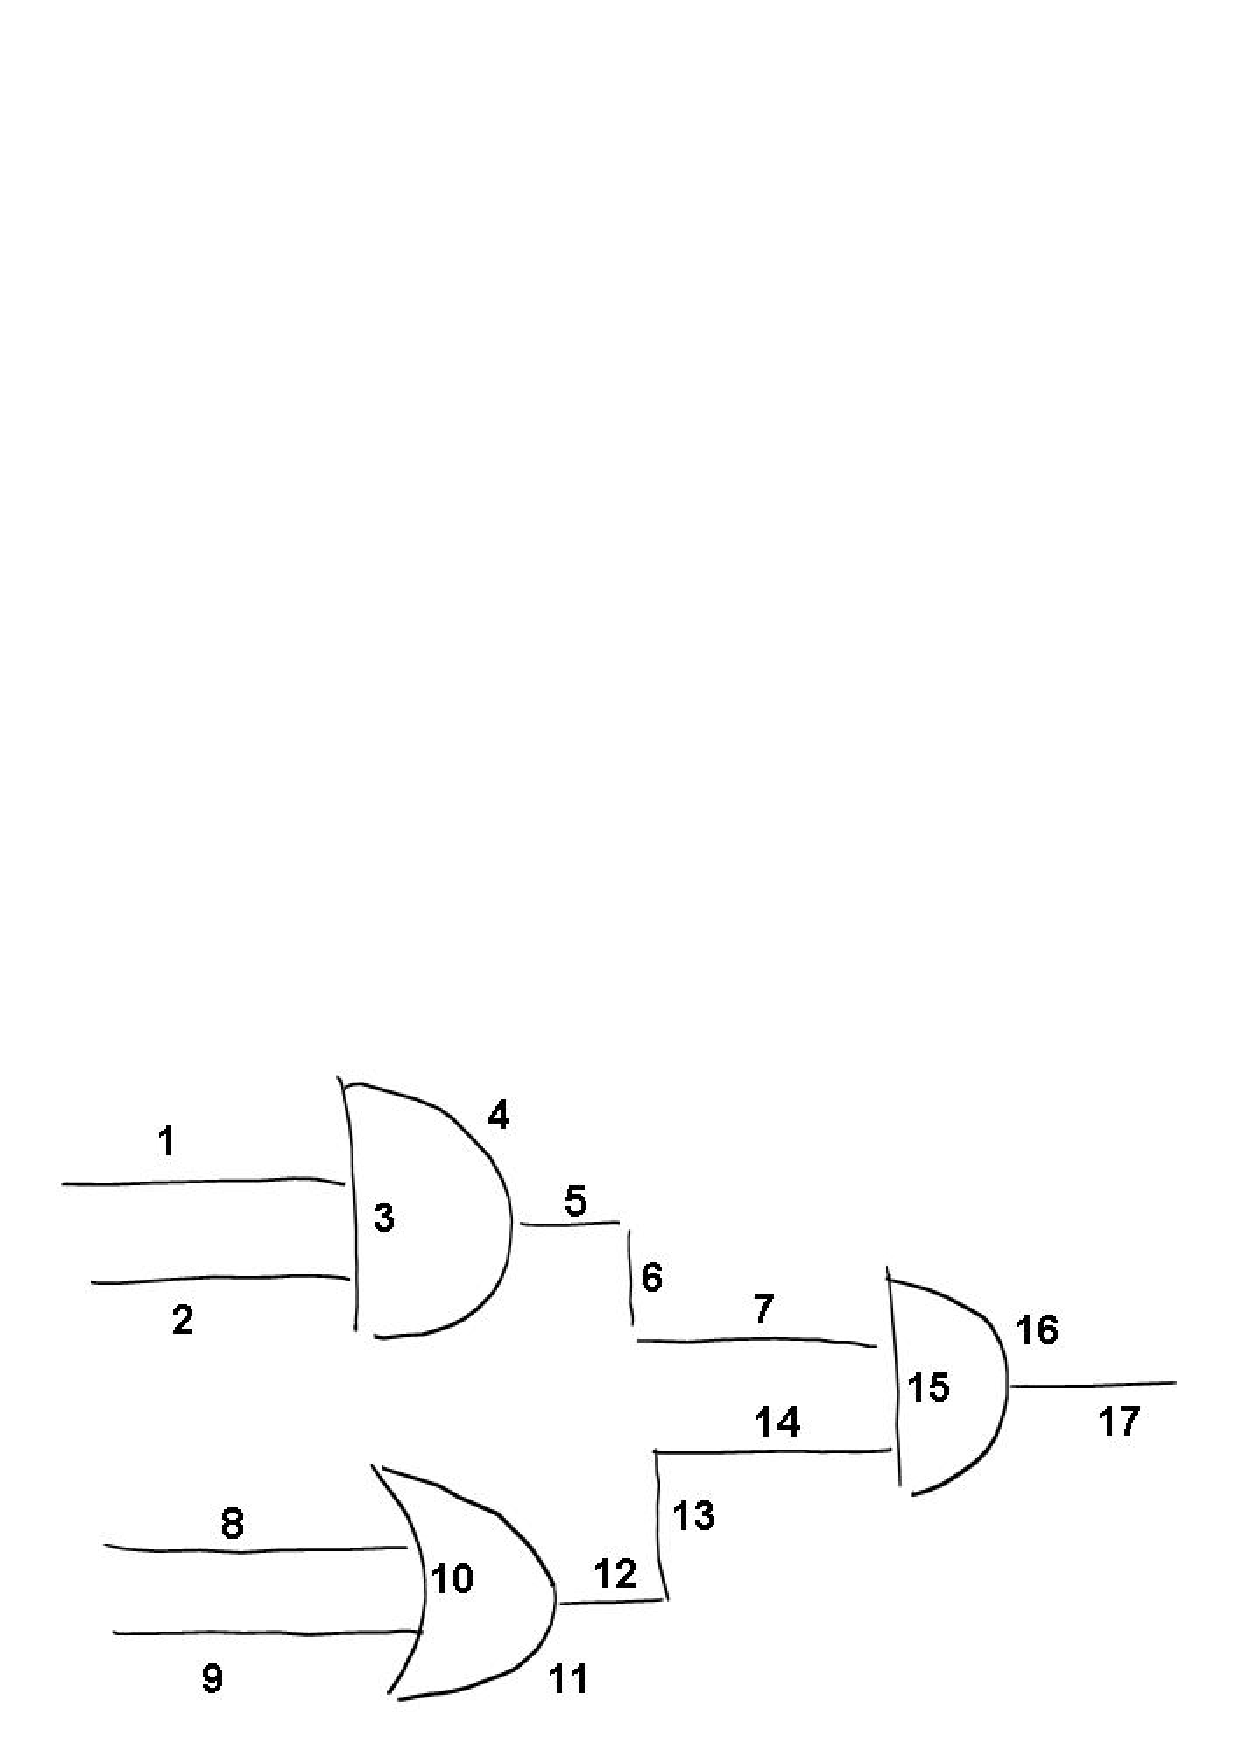
\includegraphics[width=3.0in]{nums.png}%sample.eps}
\caption{A Simple Logic Circuit Diagram}
\label{fig:simple}
\end{figure}

In our system, we actually have an additional step in sketch recognition.
Before segmentation, the preprocessed sketch goes through a Conditional Random Field (CRF).
A CRF is a graphical model that applies a label and probability to each stroke (see BLAH for implementation details).
The CRF is providing segmentation with more information, thus making the search space smaller and thus faster.
For example, the CRF may give stroke 3 the label ``AND'' with probability 90\%, while it may give stroke 13 the label ``WIRE'' with probability 60\%.
Notice that even though the CRF applies a label to each stroke, we still have not recognized the sketch.
We need to know what group of strokes make up the different components.
The CRF applies a label to an individual stroke, while segmentation and recognition applies a label to a whole component. 

Even with this extra information, by no means is segmentation trivial.
First of all, given the labelling ``AND'' to two strokes A and B with probabilities $X$ and $Y$, we cannot say that A and B are an ``AND'' gate with probability $X \times Y$ since A and B are not independent and may not even belong to the same component.
Thus, to get the probability that A and B are an ``AND'' gate, we still must use recognition.
And while the labels usually help, they can also hinder progress if they are wrong.
Segmentation should be able to take into account to account the labels, yet adjust them if they are wrong, and segment a sketch in less than exponential time.
%Why segment? So what?

\section{Approaches}
In our attempts to solve the segmentation problem, we took two different approaches.
It is necessary to make a clear distinction between the two.
While they both attempt to solve the same problem, they are not interconnected.
That said, our two approaches consist of a clustering with learned weights method and a graph theory method.

\subsection{Clustering Method}
Clustering is an unsupervised learning technique that partitions a data set based on some distance metric on the data set.
In our clustering approach we used a weighted K-Means based clustering approach.
First, K-Means must be explained.
K-Means clustering is used to partition the data into exactly K clusters (there are ways to expand K-Means to partition the data into an dynamic number of clusters).
K-Means uses cluster centers that move around in the space defined by the data set.
Initially random, the cluster centers grab the points in the data set that are closest to them (using the distance metric defined).
Then, the cluster centers update themselves, and move to the center of all the points they own.
This process repeats until all of the cluster centers are static.
The partitions of the data set are defined in the parts that make up the points that the cluster centers own.
The fitness of K-Means is the sum of all the points' distances from the cluster centers that they belong to.
While K-Means is relatively simple, it does suffer from inconsistency.
That is, from run to run on the same data set, K-Means will likely return slightly different results.
To help alleviate this problem, K-Means can be run multilpe times, and the run with the best fitness can be taken.
This is not unreasonable as K-Means is very fast.

The distance measure that commonly used in K-Means is just the Euclidean distance
$$
d(C, p) = \sqrt{\sum_{i=1}^{n} (C_i - p_i)^2},
$$
where $C$ is a cluster center and $p$ is a point in the data set.

The only difference between K-Means and our weighted K-Means is the distance metric.
We used the distance metric
$$
d(C^k, p) = \sqrt{\sum_{i=1}^{n} w_i^k (C_i^k - p_i)^2},
$$
where $C^k$ is of class $k$ and $w_i^k$ is the weighting factor for class $k$ at $i$.
That is, each cluster center can have its own set of weights.
The theory was that each particular label would have its own cluster center.
That is, we could have a cluster center for ``AND'', ``OR'', and any other label that we wanted.

To learn what weights worked best, we deployed a genetic algorithm.
A genetic algorithm is a computational method based on the theory of evolution.
First, an initial population is created.
Next, the fitness of each individual in the population is calculated (based on what is known as a fitness function).
Thirdly, those with the best fitness (or those that survive by chance) are chosen to reproduce (known as the selection).
Then the chosen population creates the next generation through what is known as crossover and mutation (known as reproduction).
Crossover is the combination of two individuals while mutation is a random change in a single individual.
This process continues until some ending condition is met.
Each step in the process is crucial.
If the fitness function is not representative of the best of the population, then you will not improve over time.
If selection is too restrictive, then you will quickly come to a population of all the same individuals.
If crossover ...
If mutation happens too often, then it will take a long time to reach a fit population.
If mutation happens too rarely, then the population will tend to get stuck at local minima.

Basically, a genetic algorithm produces a population, breeds and mutates them, and keeps some proportion of the population based on some fitness function.
The population that we used was composed of weighting vectors and the fitness function we used was the value that K-Means returned.
Our crossover was a basic, multiple point crossover.

How does it use label info... how does it further use clustering after initial... how does it use recognition...?

\subsection{Graph Theory Method}
%The graph theory method is based on the distances between pairwise combinations of strokes.
Initially, this method believes everything that the CRF labels.
Every stroke is put into a component with where all the other strokes have the same label.
From within each component, an adjacency matrix is created.
An adjaceny matrix is just an $n \times n$ matrix composed of 0's and 1's, where $n$ is the number of strokes in the component.
At $(x, y)$ a 1 indicates that strokes $x$ and $y$ are adjacent, and a 0 means that they are not adjacent.
Given to strokes $I$ and $J$ (where $i \in I$ represents the points in stroke $I$), we define the following functions:
$$
d(i, j) = \sqrt{(i_x - j_x)^2 + (i_y - j_y)^2},
$$
\[
\min(I, J) = \left\{
\begin{matrix}
\min_{i \in I, j \in J} d(i, j) & \mathrm{no\ wires}\\
\min\{
	\min_{j \in J} d(i_0, j),
	\min_{i \in I} d(i, j_0),\\
	\min_{j \in J} d(i_{last}, j),
	\min_{i \in I} d(i, j_{last})
	\} & \mathrm{else,}
\end{matrix} \right.
\]
$$
measure(I, J) = \frac{\min(I, J)}{diagonal(I) + diagonal(J) + 1},
$$
where $diagonal(I)$ is the diagonal length of the smallest bounding box around $I$.
$\min(I, J)$ is a modified minumum distance measure between two strokes.
If neither of the strokes are wires, then the first condition is met, and the absolute minimum is found by trying every combination of pairwise points.
If either of the strokes are wires, then the second condition is met, and the minimum is the distance from an endpoint to any other point on the other stroke.
Strokes $I$ and $J$ are considered adjacent if $measure(I, J) < \alpha$.
Part of the reason for using a modified distance measure is due to the nature of logic circuit diagrams.
Frequently, wires overlap and are not meant to represent the same component.
For example, see Figure~\ref{fig:adjacencies}.
Here $A\sim D$, $B\sim E$, $D\sim F$, $E\sim F$, while $B\not \sim D$, $C\not \sim D$, $C\not \sim E$ as desired.
The reason for dividing by the sum of the diagonal of the strokes $I$ and $J$ is to provide a unitless measure that is invariant under scaling.
Thus, if strokes $I$ and $J$ are adjacent, then if $I$ and $J$ are scaled by any factor, than they would still be adjacent.
We also add a small constant to the bottom of the fraction just in case we get the pathological case were both diagonals are zero.
In practice, $\alpha = [0.05, 0.10]$ is used. 

\begin{figure}[h]
\centering
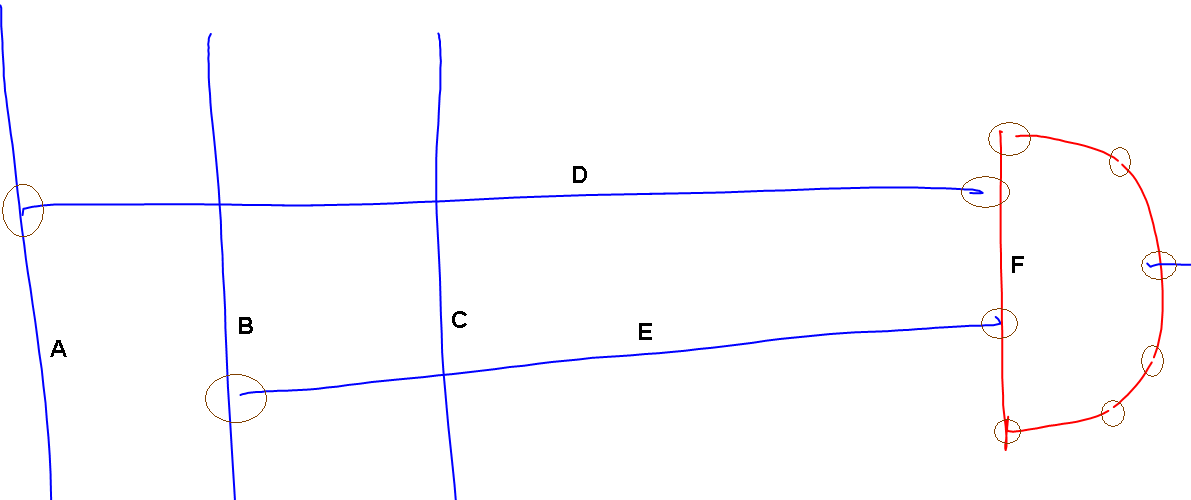
\includegraphics[width=3.0in]{adjacencies.png}%sample.eps}
\caption{Blue strokes are labeled ``WIRE'' and red strokes are labeled ``GATE''. 
Even though the wire and gate strokes are in their own component, we can still test whether or not the strokes are adjacent.}
\label{fig:adjacencies}
\end{figure}


Next, a connection matrix is made.
A connection matrix is similar to an adjacency matrix, except it determines whether two strokes are connected (that is, there is a path between the two strokes).
To create the connection matrix, a depth first search is tried on all pairwise combinations of the strokes in the component.
Depth first search works by marking the current vertex as visited, and performing depth first search on all non visited neighboring vertices (those that are adjacent to it).
This process repeats until it finds the goal, or it runs out of vertices to try.
As with the adjacency matrix, a 1 is inserted if two strokes are connected, 0 otherwise.
Once the connection matrix has been created, it is simple to find the connected components.
The connected components are all those that have the same row entry.


\begin{figure}[h]
\centering
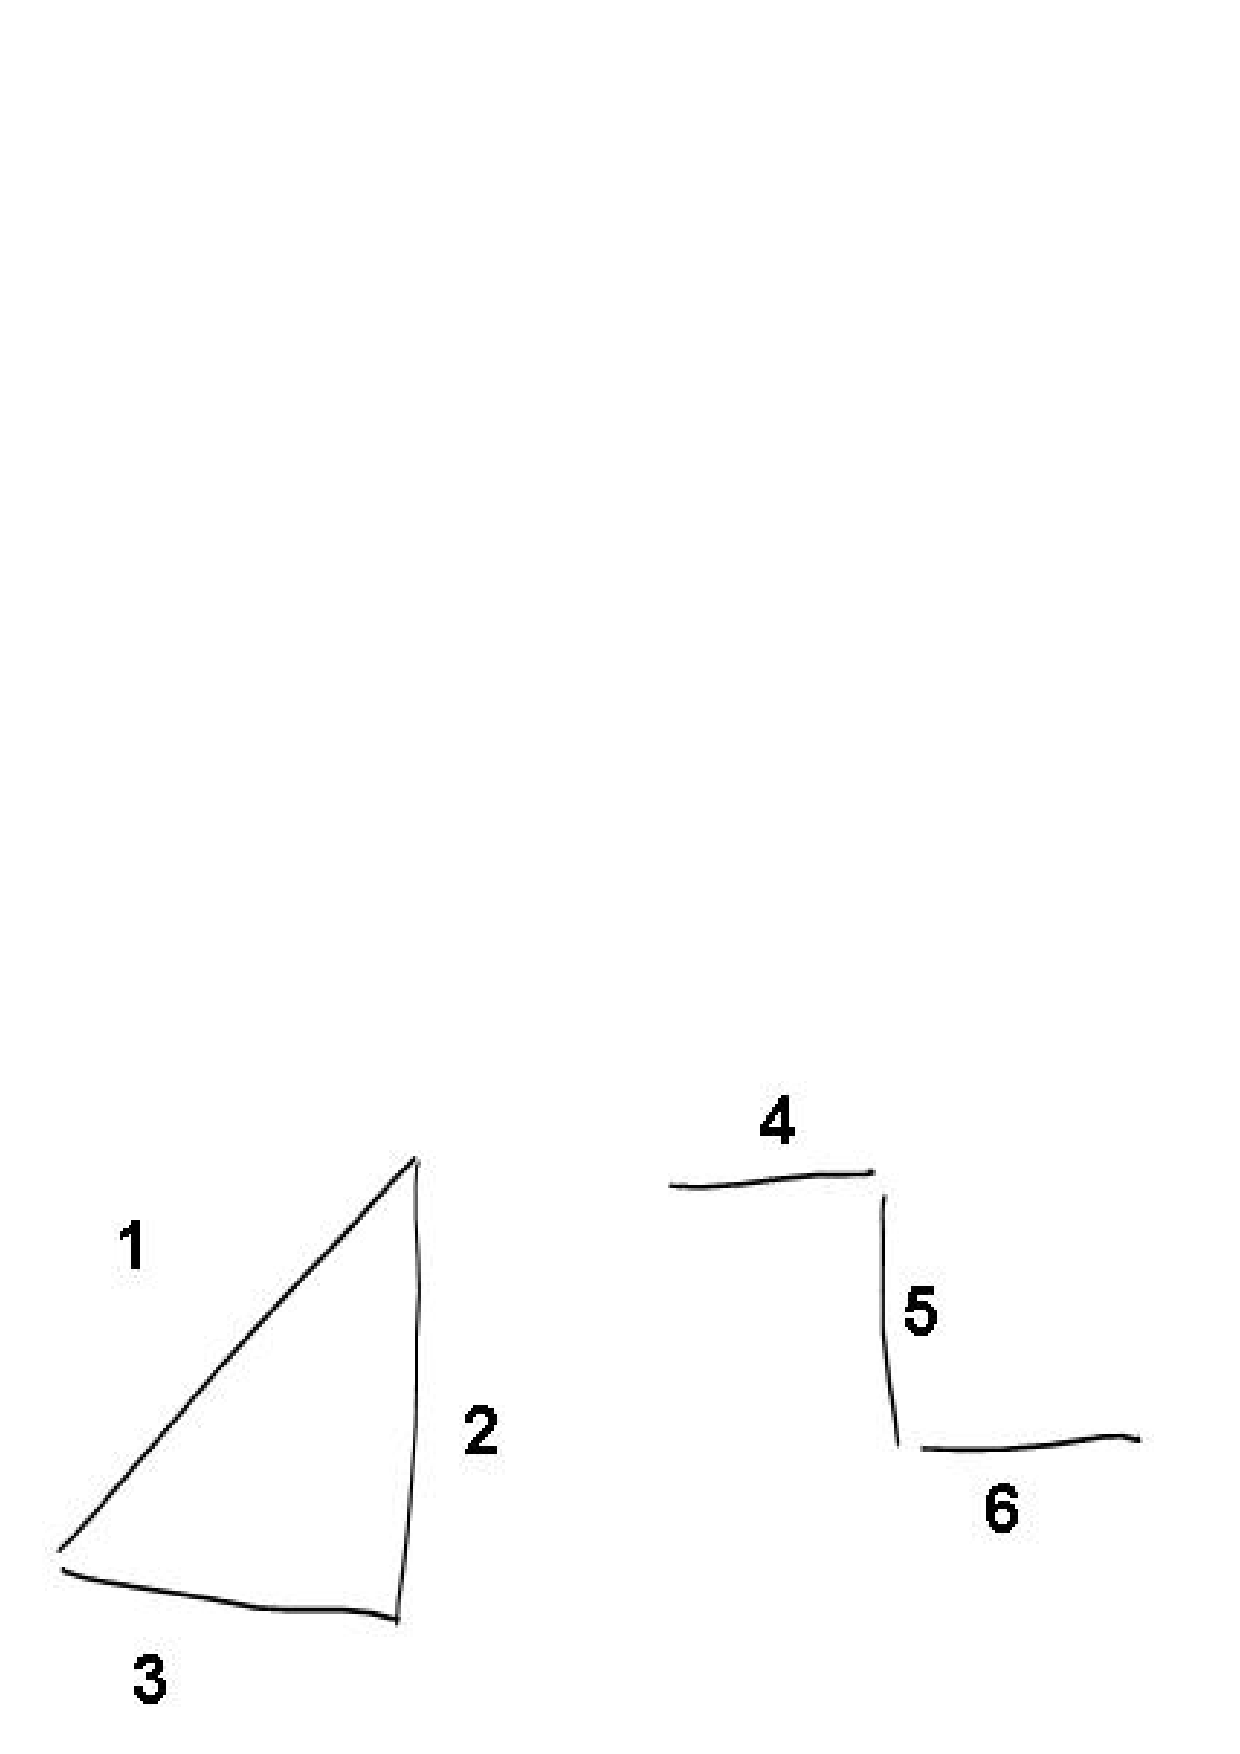
\includegraphics[width=3.0in]{connections.png}%sample.eps}
\caption{Strokes \{1 2 3\} compose a connected component as do strokes \{4 5 6\}.}
\label{fig:connections}
\end{figure}

Consider Figure~\ref{fig:connections}. 
An adjacency matrix would be
$$
\left(
\begin{array}{cccccc}
0&1&1&0&0&0\\
1&0&1&0&0&0\\
1&1&0&0&0&0\\
0&0&0&0&1&0\\
0&0&0&1&0&1\\
0&0&0&0&1&0\\
\end{array}
\right).
$$
A connection matrix would be
$$
\left(
\begin{array}{cccccc}
1&1&1&0&0&0\\
1&1&1&0&0&0\\
1&1&1&0&0&0\\
0&0&0&1&1&1\\
0&0&0&1&1&1\\
0&0&0&1&1&1\\
\end{array}
\right).
$$
Notice that rows 1, 2, and 3 are the same, and rows 4, 5, and 6 are the same.



Lorem ipsum dolor sit amet, consectetur adipisicing elit, sed do eiusmod tempor incididunt ut labore et dolore magna aliqua. Ut enim ad minim veniam, quis nostrud exercitation ullamco laboris nisi ut aliquip ex ea commodo consequat. Duis aute irure dolor in reprehenderit in voluptate velit esse cillum dolore eu fugiat nulla pariatur. Excepteur sint occaecat cupidatat non proident, sunt in culpa qui officia deserunt mollit anim id est laborum.

Lorem ipsum dolor sit amet, consectetur adipisicing elit, sed do eiusmod tempor incididunt ut labore et dolore magna aliqua. Ut enim ad minim veniam, quis nostrud exercitation ullamco laboris nisi ut aliquip ex ea commodo consequat. Duis aute irure dolor in reprehenderit in voluptate velit esse cillum dolore eu fugiat nulla pariatur. Excepteur sint occaecat cupidatat non proident, sunt in culpa qui officia deserunt mollit anim id est laborum.

Lorem ipsum dolor sit amet, consectetur adipisicing elit, sed do eiusmod tempor incididunt ut labore et dolore magna aliqua. Ut enim ad minim veniam, quis nostrud exercitation ullamco laboris nisi ut aliquip ex ea commodo consequat. Duis aute irure dolor in reprehenderit in voluptate velit esse cillum dolore eu fugiat nulla pariatur. Excepteur sint occaecat cupidatat non proident, sunt in culpa qui officia deserunt mollit anim id est laborum.

Lorem ipsum dolor sit amet, consectetur adipisicing elit, sed do eiusmod tempor incididunt ut labore et dolore magna aliqua. Ut enim ad minim veniam, quis nostrud exercitation ullamco laboris nisi ut aliquip ex ea commodo consequat. Duis aute irure dolor in reprehenderit in voluptate velit esse cillum dolore eu fugiat nulla pariatur. Excepteur sint occaecat cupidatat non proident, sunt in culpa qui officia deserunt mollit anim id est laborum.

Clustering with learned Weights
\begin{itemize}
\item What is clustering?
\item What is a genetic algorithm?
\item Discuss how the two have been used in similar context before.
\end{itemize}

Graph based method
\begin{itemize}
\item What is this method?
\item How has it been done before? put in beginning
\item What is unique about our approach? (Segmentation supplamented with CRF info)
\end{itemize}

\section{Results and Discussion}
Lorem ipsum dolor sit amet, consectetur adipisicing elit, sed do eiusmod tempor incididunt ut labore et dolore magna aliqua. Ut enim ad minim veniam, quis nostrud exercitation ullamco laboris nisi ut aliquip ex ea commodo consequat. Duis aute irure dolor in reprehenderit in voluptate velit esse cillum dolore eu fugiat nulla pariatur. Excepteur sint occaecat cupidatat non proident, sunt in culpa qui officia deserunt mollit anim id est laborum.

Lorem ipsum dolor sit amet, consectetur adipisicing elit, sed do eiusmod tempor incididunt ut labore et dolore magna aliqua. Ut enim ad minim veniam, quis nostrud exercitation ullamco laboris nisi ut aliquip ex ea commodo consequat. Duis aute irure dolor in reprehenderit in voluptate velit esse cillum dolore eu fugiat nulla pariatur. Excepteur sint occaecat cupidatat non proident, sunt in culpa qui officia deserunt mollit anim id est laborum.

Lorem ipsum dolor sit amet, consectetur adipisicing elit, sed do eiusmod tempor incididunt ut labore et dolore magna aliqua. Ut enim ad minim veniam, quis nostrud exercitation ullamco laboris nisi ut aliquip ex ea commodo consequat. Duis aute irure dolor in reprehenderit in voluptate velit esse cillum dolore eu fugiat nulla pariatur. Excepteur sint occaecat cupidatat non proident, sunt in culpa qui officia deserunt mollit anim id est laborum.

\begin{itemize}
\item How well did clustering work? 
\item Give actual numbers of how it didn't span multiple document
\item What was learned about clustering for segmentation?
\item How well did graph theory method work? 
\item Give estimates for initial overfitting/underfitting components. (Only as good (initially) as CRF gives us)
\end{itemize}

\section{Related Work}

In~\cite{dietrich95weighting} we see weighted features with the nearest neighbor algorithm.
In~\cite{demiroz96genetic} we see learning weights for nearest neighbor using genetic algorithms.
In~\cite{spatial} we see a simiilar graph theory method but it is different.

\section{Future Work}
Lorem ipsum dolor sit amet, consectetur adipisicing elit, sed do eiusmod tempor incididunt ut labore et dolore magna aliqua. Ut enim ad minim veniam, quis nostrud exercitation ullamco laboris nisi ut aliquip ex ea commodo consequat. Duis aute irure dolor in reprehenderit in voluptate velit esse cillum dolore eu fugiat nulla pariatur. Excepteur sint occaecat cupidatat non proident, sunt in culpa qui officia deserunt mollit anim id est laborum.

Lorem ipsum dolor sit amet, consectetur adipisicing elit, sed do eiusmod tempor incididunt ut labore et dolore magna aliqua. Ut enim ad minim veniam, quis nostrud exercitation ullamco laboris nisi ut aliquip ex ea commodo consequat. Duis aute irure dolor in reprehenderit in voluptate velit esse cillum dolore eu fugiat nulla pariatur. Excepteur sint occaecat cupidatat non proident, sunt in culpa qui officia deserunt mollit anim id est laborum.

Lorem ipsum dolor sit amet, consectetur adipisicing elit, sed do eiusmod tempor incididunt ut labore et dolore magna aliqua. Ut enim ad minim veniam, quis nostrud exercitation ullamco laboris nisi ut aliquip ex ea commodo consequat. Duis aute irure dolor in reprehenderit in voluptate velit esse cillum dolore eu fugiat nulla pariatur. Excepteur sint occaecat cupidatat non proident, sunt in culpa qui officia deserunt mollit anim id est laborum.

Lorem ipsum dolor sit amet, consectetur adipisicing elit, sed do eiusmod tempor incididunt ut labore et dolore magna aliqua. Ut enim ad minim veniam, quis nostrud exercitation ullamco laboris nisi ut aliquip ex ea commodo consequat. Duis aute irure dolor in reprehenderit in voluptate velit esse cillum dolore eu fugiat nulla pariatur. Excepteur sint occaecat cupidatat non proident, sunt in culpa qui officia deserunt mollit anim id est laborum.

\begin{itemize}
\item Additional testing for clustering? Different features? More relative features than absolute?
\item Shape based recognizer that gives a percentage for belief... possibly a SVM one like HHRECO.
\item Incorporate recognizer into segmenter.
\item Build recognizer
\item Build connectedness... determines how all the segments interact... can be part of segmenter
\end{itemize}

\section{Conclusion}


\bibliographystyle{acmsiggraph}
\nocite{*}
\bibliography{devin}
\end{document}
